% Copyright 2004 by Till Tantau <tantau@users.sourceforge.net>.
%
% In principle, this file can be redistributed and/or modified under
% the terms of the GNU Public License, version 2.
%
% However, this file is supposed to be a template to be modified
% for your own needs. For this reason, if you use this file as a
% template and not specifically distribute it as part of a another
% package/program, I grant the extra permission to freely copy and
% modify this file as you see fit and even to delete this copyright
% notice. 

\documentclass[aspectratio=169]{beamer}
\usepackage{pagecolor}
\usepackage[export]{adjustbox}
\usepackage{float}
\usepackage{graphicx}
\graphicspath{{Figures/}}
\usepackage{subcaption}

% There are many different themes available for Beamer. A comprehensive
% list with examples is given here:
% http://deic.uab.es/~iblanes/beamer_gallery/index_by_theme.html
% You can uncomment the themes below if you would like to use a different
% one:
%\usetheme{AnnArbor}
%\usetheme{Antibes}
%\usetheme{Bergen}
%\usetheme{Berkeley}
%\usetheme{Berlin}
%\usetheme{Boadilla}
%\usetheme{boxes}
%\usetheme{CambridgeUS}
%\usetheme{Copenhagen}
%\usetheme{Darmstadt}
\usetheme{default}
%\usetheme{Frankfurt}
%\usetheme{Goettingen}
%\usetheme{Hannover}
%\usetheme{Ilmenau}
%\usetheme{JuanLesPins}
%\usetheme{Luebeck}
%\usetheme{Madrid}
%\usetheme{Malmoe}
%\usetheme{Marburg}
%\usetheme{Montpellier}
%\usetheme{PaloAlto}
%\usetheme{Pittsburgh}
%\usetheme{Rochester}
%\usetheme{Singapore}
%\usetheme{Szeged}
%\usetheme{Warsaw}


\title{Langevin Monte Carlo}

% A subtitle is optional and this may be deleted
% \subtitle{Optional Subtitle}

\author{Bowen Han\inst{1} \and Matthew Holden\inst{1} \and Marko Puza\inst{1} \and Tom Hodgson\inst{1}\\ \textit{Supervised by:} Sotirios Sabanis\inst{2}}
% - Give the names in the same order as the appear in the paper.
% - Use the \inst{?} command only if the authors have different
%   affiliation.

\institute[Universities of Somewhere and Elsewhere] % (optional, but mostly needed)
{
  \inst{1}%
    The Maxwell Institute Graduate School in Analysis \& its Applications
  \and
  \inst{2}%
  University of Edinburgh
}
% - Use the \inst command only if there are several affiliations.
% - Keep it simple, no one is interested in your street address.

\date{ Interim Taster Project Presentation, 01/03/2019}
% - Either use conference name or its abbreviation.
% - Not really informative to the audience, more for people (including
%   yourself) who are reading the slides online

% \subject{Theoretical Computer Science}
% This is only inserted into the PDF information catalog. Can be left
% out. 

% If you have a file called "university-logo-filename.xxx", where xxx
% is a graphic format that can be processed by latex or pdflatex,
% resp., then you can add a logo as follows:

% \pgfdeclareimage[height=0.5cm]{university-logo}{university-logo-filename}
% \logo{\pgfuseimage{university-logo}}

% Delete this, if you do not want the table of contents to pop up at
% the beginning of each subsection:
% \AtBeginSubsection[]
% {
%   \begin{frame}<beamer>{Outline}
%     \tableofcontents[currentsection,currentsubsection]
%   \end{frame}
% }

% Let's get started
\begin{document}

\setbeamercolor{background canvas}{bg=white}
\begin{frame}
  \titlepage
\end{frame}

% \begin{frame}{Outline}
%   \tableofcontents
%   % You might wish to add the option [pausesections]
% \end{frame}

% Section and subsections will appear in the presentation overview
% and table of contents.
\section{Horse-Racing}


\subsection{TULA paper}

\begin{frame}{Frame Title}
    
\end{frame}

\begin{frame}{First and Second Moments of Double Well - \(h=0.01\)}%{Optional Subtitle}
        \begin{figure}[h]
        \centering
        \begin{minipage}{0.5\linewidth}
          \centering
          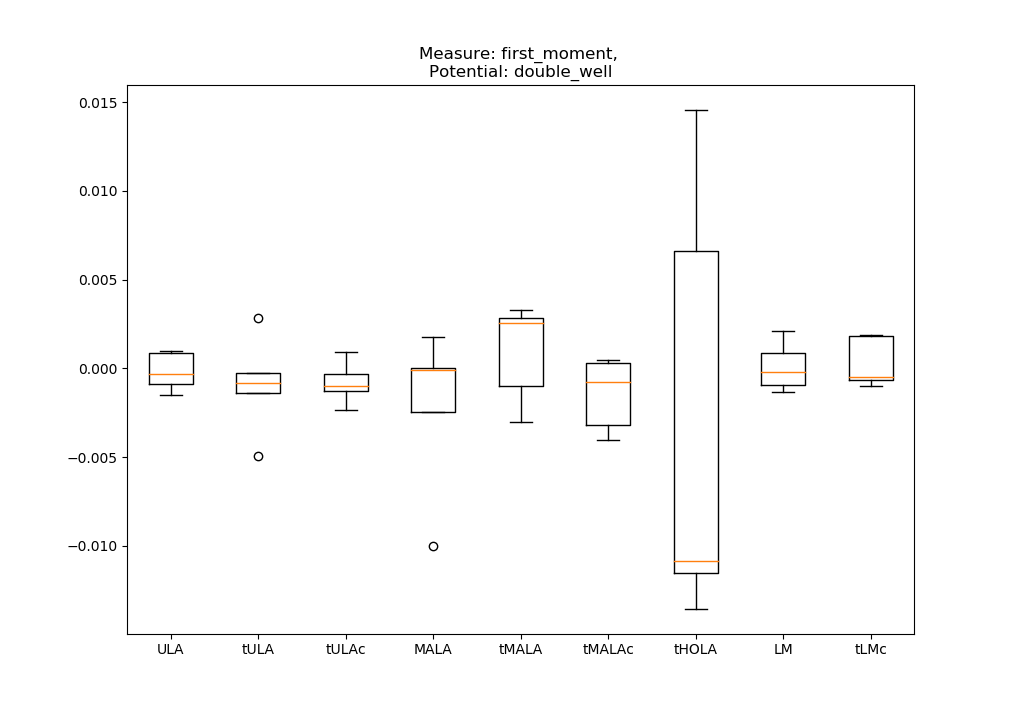
\includegraphics[width=0.99\linewidth]{10sBoxPlot1moment100dim001step.png}
        \end{minipage}%
        \begin{minipage}{0.5\linewidth}
          \centering
          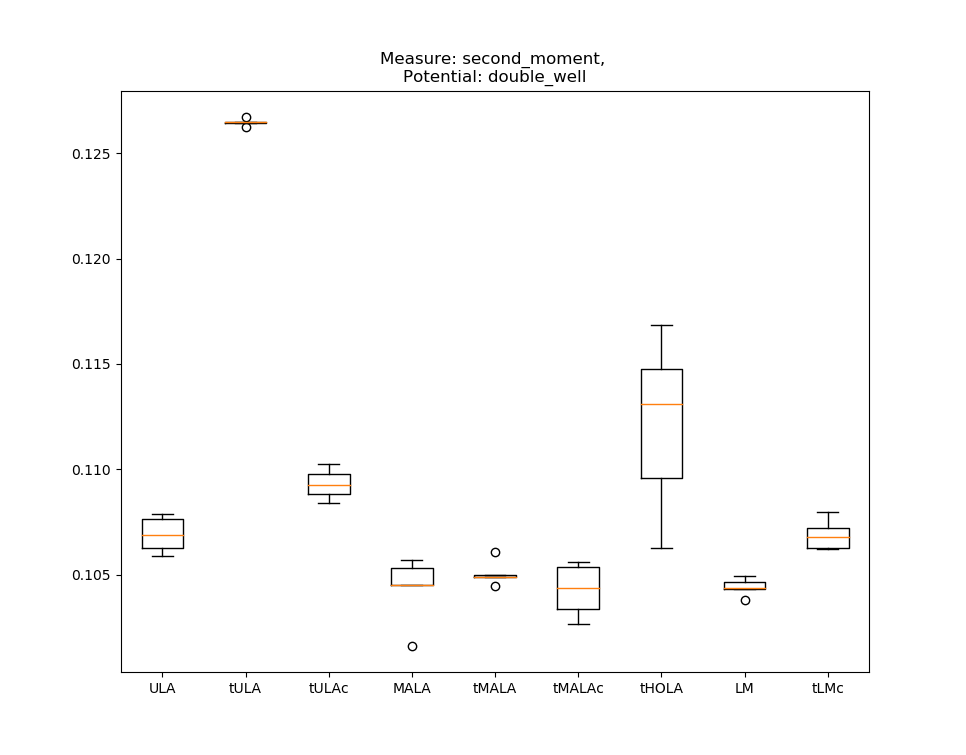
\includegraphics[width=0.99\linewidth]{10sBoxPlot2moment100dim001step.png}
        \end{minipage}%
        \end{figure}
\end{frame}

\begin{frame}{First and Second Moments of Double Well - \(h=0.1\)}%{Optional Subtitle}
        \begin{figure}[h]
        \centering
        \begin{minipage}{0.5\linewidth}
          \centering
          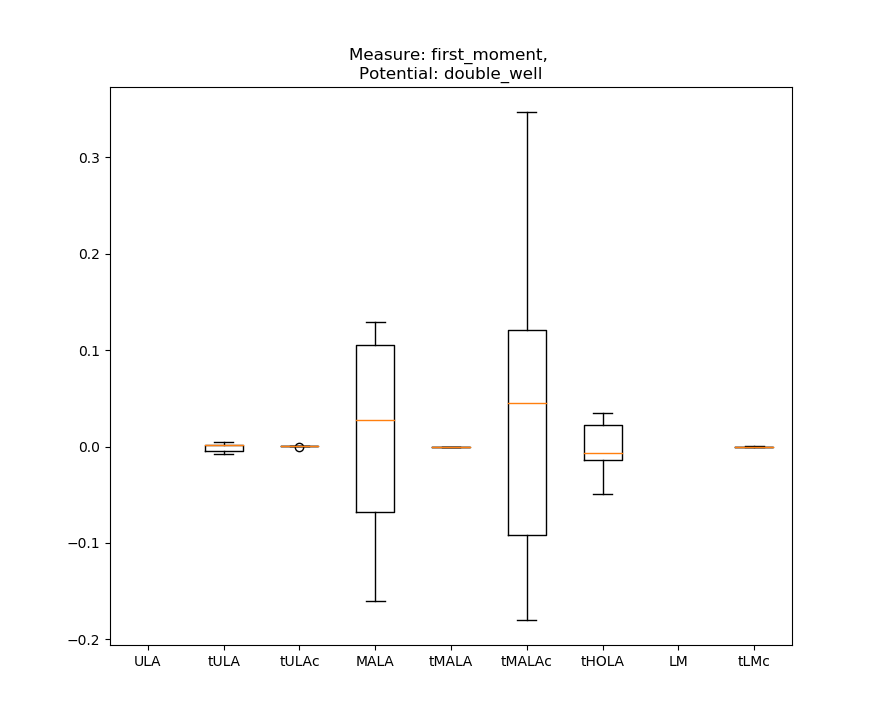
\includegraphics[width=0.99\linewidth]{10sBoxPlot1moment100dim01step.png}
        \end{minipage}%
        \begin{minipage}{0.5\linewidth}
          \centering
          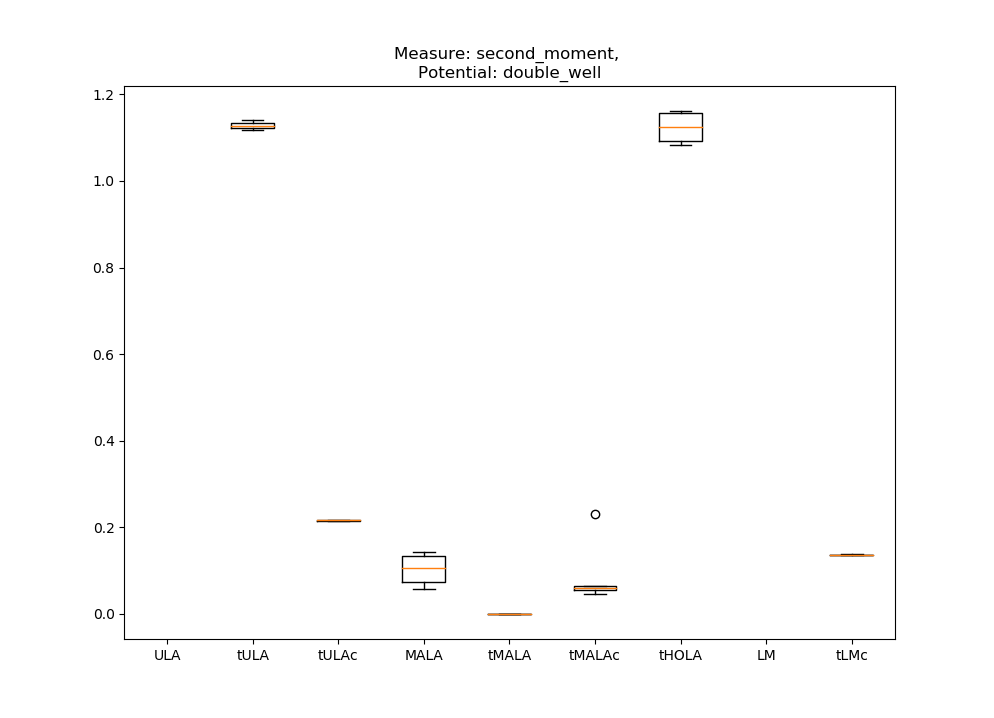
\includegraphics[width=0.99\linewidth]{10sBoxPlot2moment100dim01step.png}
        \end{minipage}%
        \end{figure}
\end{frame}



\begin{frame}{First and Second Moments of Ill-Condition Gaussian - 1st Dimension}%{Optional Subtitle}
        \begin{figure}[h]
        \centering
        \begin{minipage}{0.5\linewidth}
          \centering
          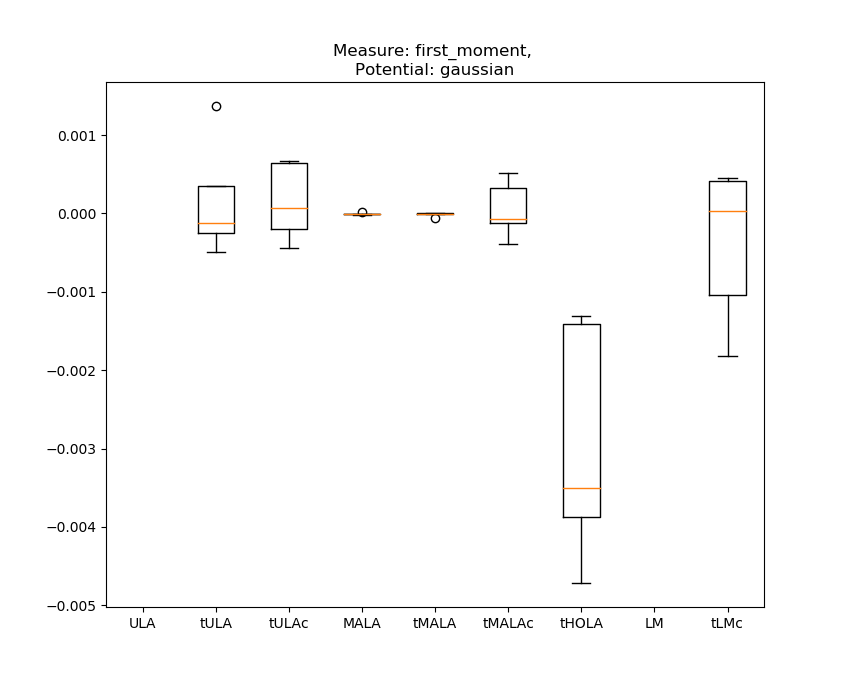
\includegraphics[width=0.99\linewidth]{illcond10sBoxPlot1moment100dim01step.png}
        \end{minipage}%
        \begin{minipage}{0.5\linewidth}
          \centering
          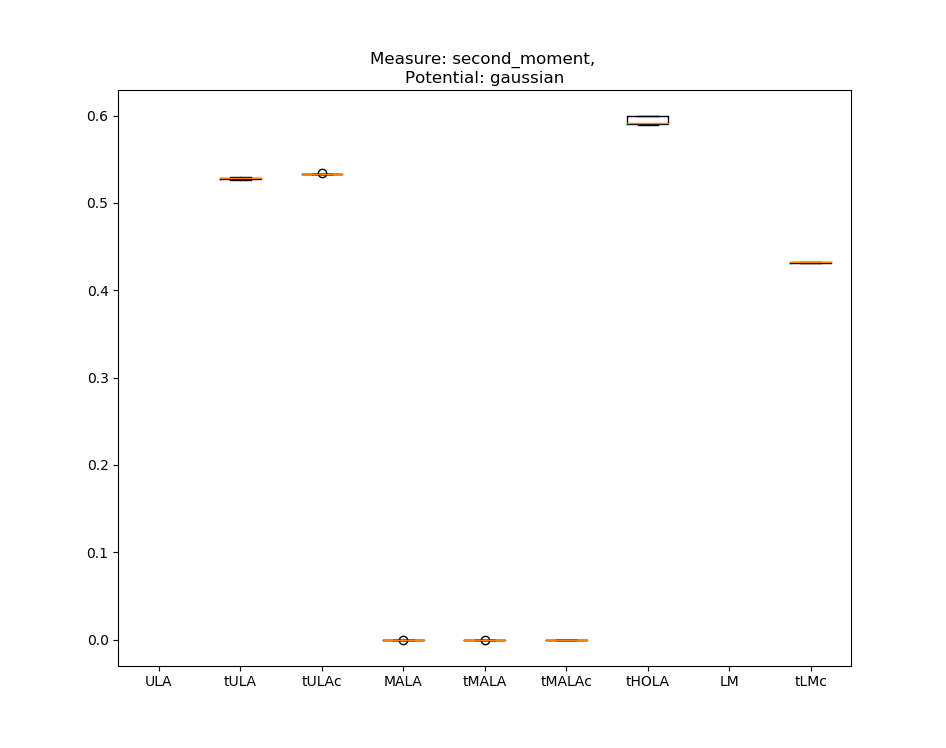
\includegraphics[width=0.99\linewidth]{illcond10sBoxPlot2moment100dim01step.png}
        \end{minipage}%
        \end{figure}
\end{frame}

\begin{frame}{First and Second Moments of Ill-Condition Gaussian - 2nd Dimension}%{Optional Subtitle}
        \begin{figure}[h]
        \centering
        \begin{minipage}{0.5\linewidth}
          \centering
          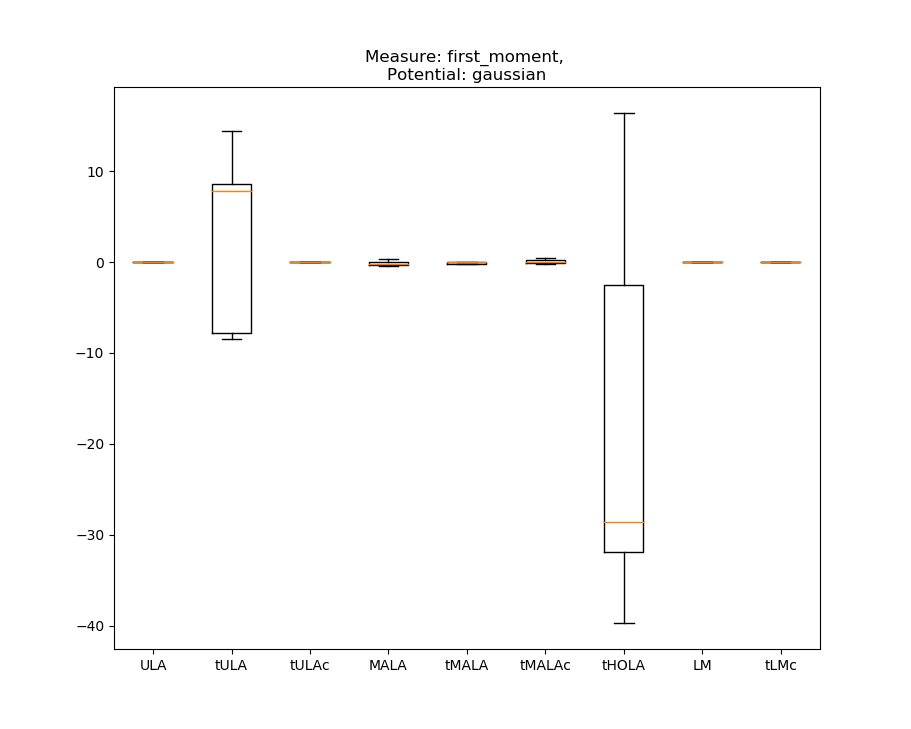
\includegraphics[width=0.99\linewidth]{illcond10sBoxPlot1moment100dim01step2nddim.png}
        \end{minipage}%
        \begin{minipage}{0.5\linewidth}
          \centering
          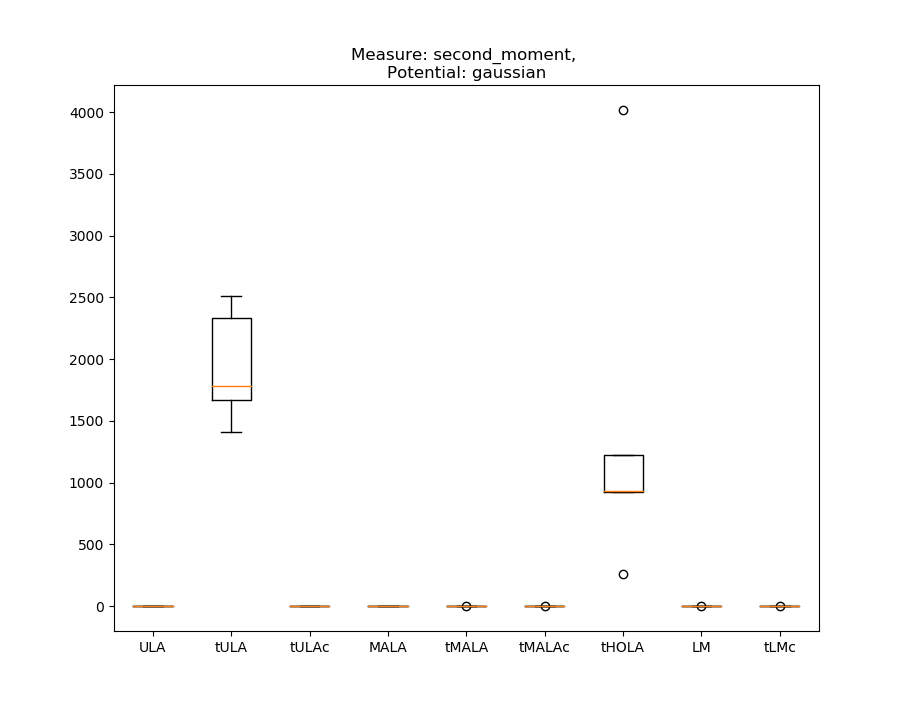
\includegraphics[width=0.99\linewidth]{illcond10sBoxPlot2moment100dim01step2nddim.png}
        \end{minipage}%
        \end{figure}
\end{frame}
\begin{frame}{First and Second Moments of Ill-Condition Gaussian - 2nd Dimension}%{Optional Subtitle}
        \begin{figure}[h]
        \centering
        \begin{minipage}{0.7\linewidth}
          \centering
          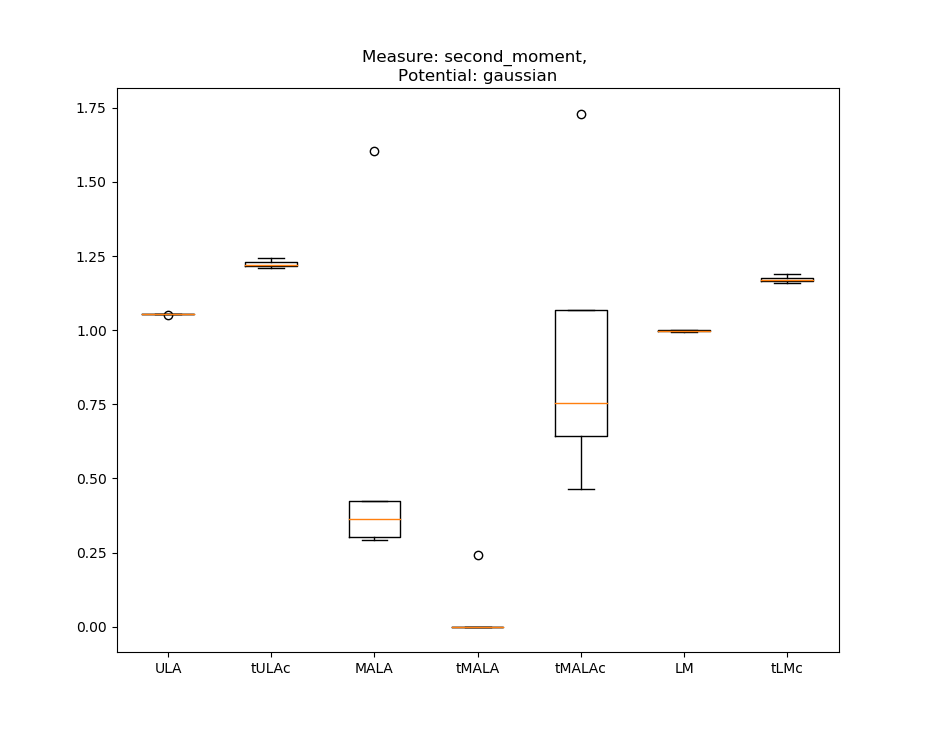
\includegraphics[width=0.99\linewidth]{illcond10sBoxPlot2moment100dim01step2nddimnotula.png}
        \end{minipage}%
        \end{figure}
\end{frame}



\subsection{Non-asymptotic behaviour}
\begin{frame}{Beyond Moments}
\begin{itemize}
    \item Total Variation
        \[\|\mu-\nu\|_{TV} - \sup_{\|f\|\leq 1} |\mu(f) - \nu(f)|\ \]
    \item Wasserstein Distance
       \[W_2(\mu,\nu) = \left( \inf_{\gamma \in \Gamma(\mu,\nu)} \int_{M\times M} d(x,y)^2 \mathrm{d}\gamma(x,y)\right)^{\frac{1}{2}}\]
\end{itemize}

\end{frame}

\begin{frame}{Durmus--Moulines Bounds}
\begin{figure}[h]
    \centering
    \begin{subfigure}[b]{\textwidth}
        \centering
        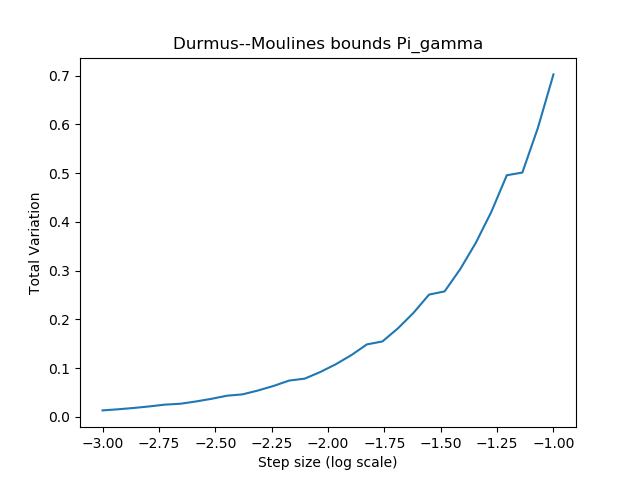
\includegraphics[width=0.23\textwidth]{Pi_gamma.png}
        \caption{Error in $\pi_\gamma$ (Choose suitable step size)}
    \end{subfigure}

\end{figure}
\begin{figure}[h]
    \centering
    \begin{subfigure}[b]{0.23\textwidth}
        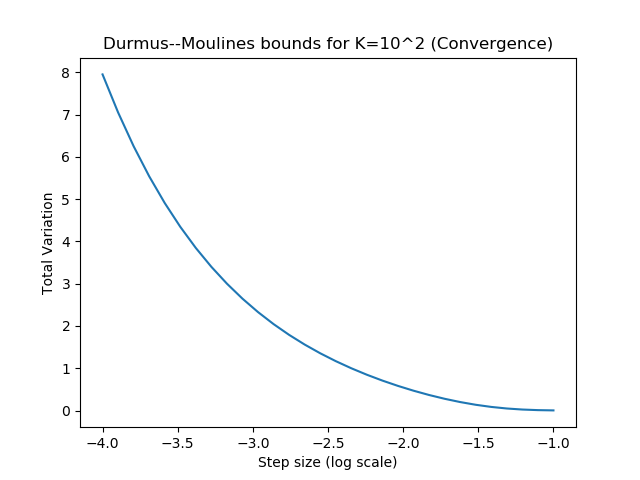
\includegraphics[width=\textwidth]{ConvergenceK1e2.png}
        \caption{K=$10^2$}
    \end{subfigure}
    ~ %add desired spacing between images, e. g. ~, \quad, \qquad, \hfill etc. 
      %(or a blank line to force the subfigure onto a new line)
    \begin{subfigure}[b]{0.23\textwidth}
        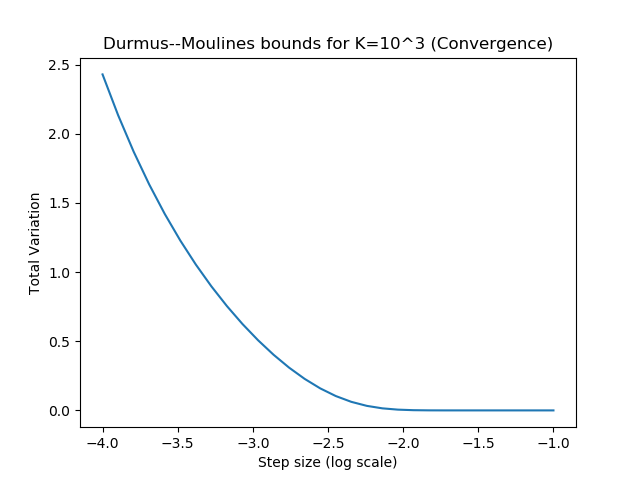
\includegraphics[width=\textwidth]{ConvergenceK1e3.png}
        \caption{K=$10^3$}
    \end{subfigure}
    ~ %add desired spacing between images, e. g. ~, \quad, \qquad, \hfill etc. 
    %(or a blank line to force the subfigure onto a new line)
    \begin{subfigure}[b]{0.23\textwidth}
        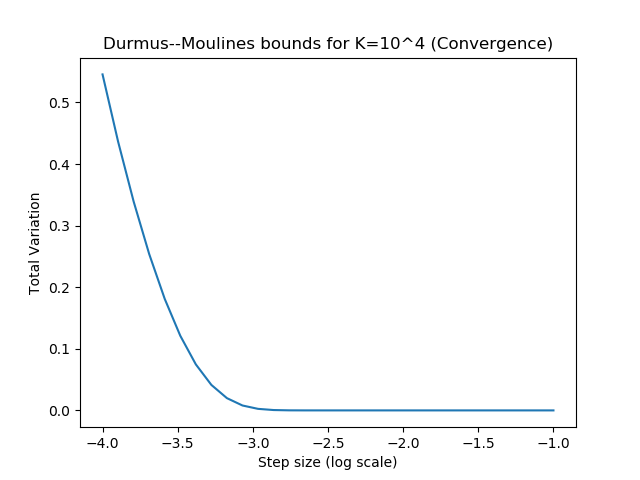
\includegraphics[width=\textwidth]{ConvergenceK1e4.png}
        \caption{K=$10^4$}
    \end{subfigure}
    ~
    \begin{subfigure}[b]{0.23\textwidth}
        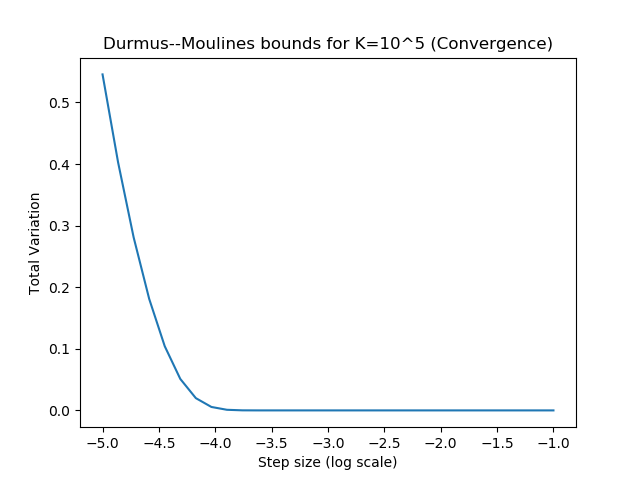
\includegraphics[width=\textwidth]{ConvergenceK1e5.png}
        \caption{K=$10^5$}
    \end{subfigure}
    
\end{figure}
\end{frame}

\subsection{Future}

\begin{frame}{Future Work}
\begin{itemize}
    \item Check Dalalyan's new `user-friendly' bound
    \item Are these bounds anywhere near sharp?
    \item Test against SGLD
    \item Test on real data
\end{itemize}
    
\end{frame}

% You can reveal the parts of a slide one at a time
% with the \pause command:
% \begin{frame}{Second Slide Title}
%   \begin{itemize}
%   \item {
%     First item.
%     \pause % The slide will pause after showing the first item
%   }
%   \item {   
%     Second item.
%   }
%   % You can also specify when the content should appear
%   % by using <n->:
%   \item<3-> {
%     Third item.
%   }
%   \item<4-> {
%     Fourth item.
%   }
%   % or you can use the \uncover command to reveal general
%   % content (not just \items):
%   \item<5-> {
%     Fifth item. \uncover<6->{Extra text in the fifth item.}
%   }
%   \end{itemize}
 % \end{frame}




\end{document}


